
Let $u_0(x) = (x-x^2) \left(\sin(3\pi x)\right)^2$. Note that, for $n=1,2,\ldots$,
\[
\int_0^1\sqrt{2}u_0(x)\sin(n\pi x)\,dx =\left\{ \begin{array}{cl} \displaystyle{{432\sqrt{2} (n^4-18n^2 + 216) \over (36n-n^3)^3 \pi^3}} & \mbox{if }n\mbox{ is odd}; \\0 & \mbox{if }n\mbox{ is even}.
\end{array}\right.
\]
Consider the problem of finding the solution $u(x,t)$ to the the fourth order partial differential equation
\[
u_t(x,t) = u_{xx}(x,t) - u_{xxxx}(x,t),\quad 0<x<1,\quad t>0
\]
with so-called hinged boundary conditions
\[
u(0,t) = u_{xx}(0,t) = u(1,t) = u_{xx}(1,t) = 0,\quad t\ge0
\]
and initial condition
\[
u(x,0) = u_0(x),\quad 0<x<1.
\]
This equation is related to a model that arises in the study of thin films. Let
\[
C^4_H[0,1] = \{ v \in C^4[0,1]:\, v(0)=v''(0)=v(1)=v''(1)=0\}.
\]
Let the linear operator $L: C^4_H[0,1] \rightarrow C[0,1]$ be defined by
\[
Lv = -v'' + v''''.
\]
\\
\begin{enumerate}
\item The operator $L$ has eigenvalues $\lambda_n\in\R$ and eigenfunctions
\[
\psi_n(x) = \sqrt{2} \sin(n \pi x)
\]
for $n = 1,2,\ldots$, which are such that
\[
L\psi_n=\lambda_n\psi_n
\]
for $n = 1,2,\ldots$. Obtain a formula for $\lambda_n$ for $n = 1,2,\ldots$.
\\
\item We can write
\[
u(x,t)=\sum_{n=1}^\infty a_n(t)\psi_n(x).
\]
What ordinary differential equation and initial condition does $a_n(t)$ satisfy for $n = 1,2,\ldots$?
\\
\item Obtain an expression for $a_n(t)$ for $n=1,2,\ldots$.
\\
\item Use you answer to part~(c) to write out a formula for $u(x,t)$.
\\
\item Let
\[
u_N(x,t)=\sum_{n=1}^N a_n(t)\psi_n(x).
\]
For each time $t=0,10^{-5},2\times 10^{-5},4 \times 10^{-5}$, produce a plot comparing
$u_1(x,t)$, $u_3(x,t)$, $u_5(x,t)$, $u_7(x,t)$ and $u_9(x,t)$. For example, at time $t=0$, your plot should appear as shown below.

\begin{center}
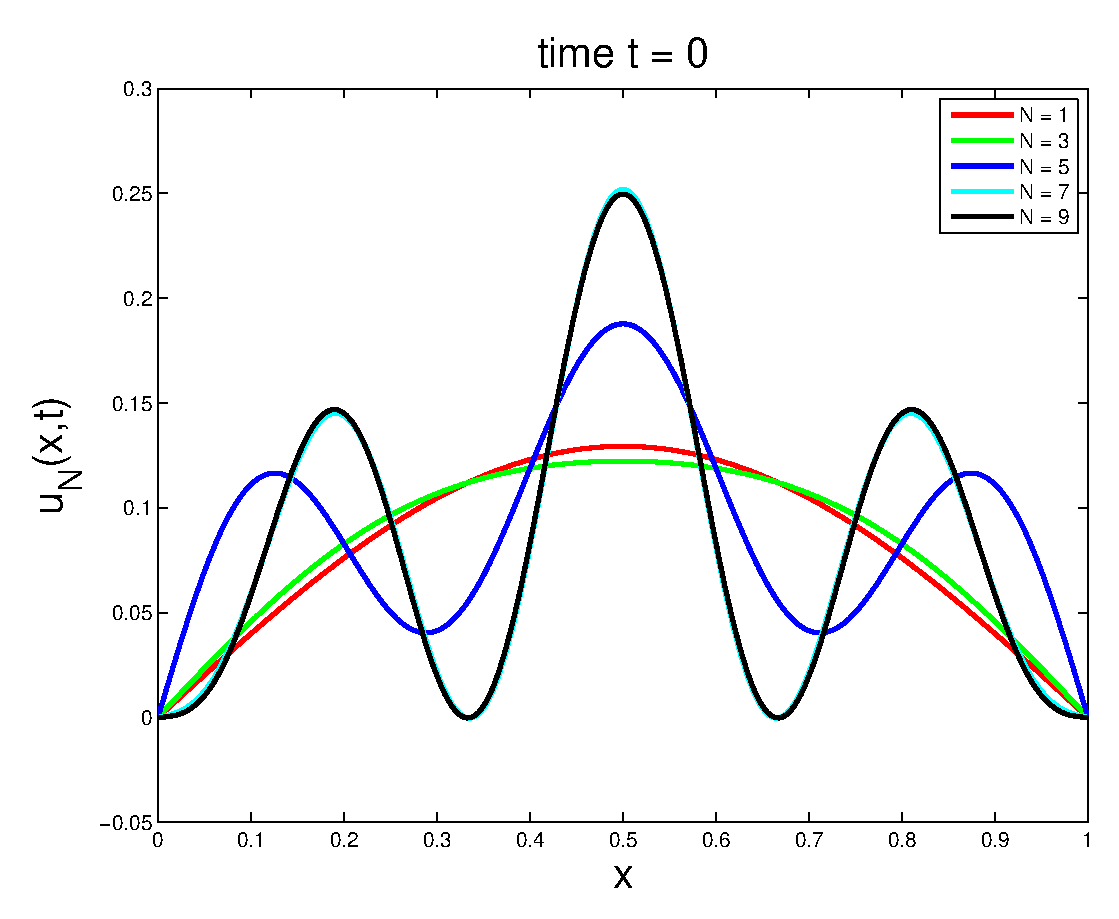
\includegraphics[scale=0.5]{fourth_a}
\end{center}

\end{enumerate}


%%%%%%%%%%%%%%%%%%%%%%%%%%%%%%%%%%%%%%%%%%%%%%%%%%%%%%%%%%%%%%%%%%%%%%%%%%%%%%%%

\ifthenelse{\boolean{showsols}}{\input fourth_sol}{}

